\chapter{Clustering Spectral Images}
\label{ch:spectra_image_clustering}

\begin{wrapfigure}{o}{0.63\textwidth}
    \centering
    \vspace{-3.3cm}
    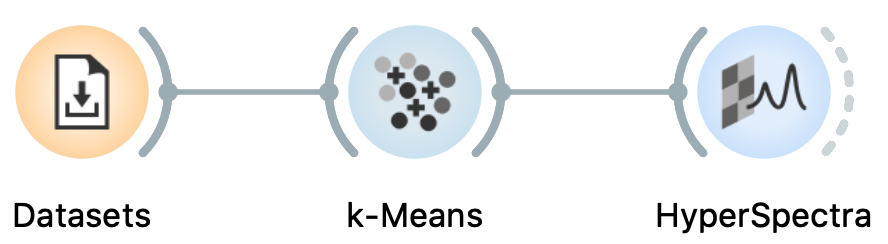
\includegraphics[width=0.75\textwidth]{graphics/ch-spectra_image_clustering/sp_image_clustering-fig1.png}
    \label{fig:spectra_image_clustering-fig1}
\end{wrapfigure}

We have already seen hierarchical clustering. Another clustering algorithm, k-Means, is much faster for data with lots of rows, like images, which contain a row (a spectrum) for each pixel. Still, for the liver-cirrhosis data, both approaches are fast. Here, we use \widget{k-Means} with k=3 clusters. 

\begin{figure}[h]
\vspace{-0.5cm}
\hspace{-1cm}\stackinset{r}{-1.15\linewidth}{t}{0.025\linewidth}
  {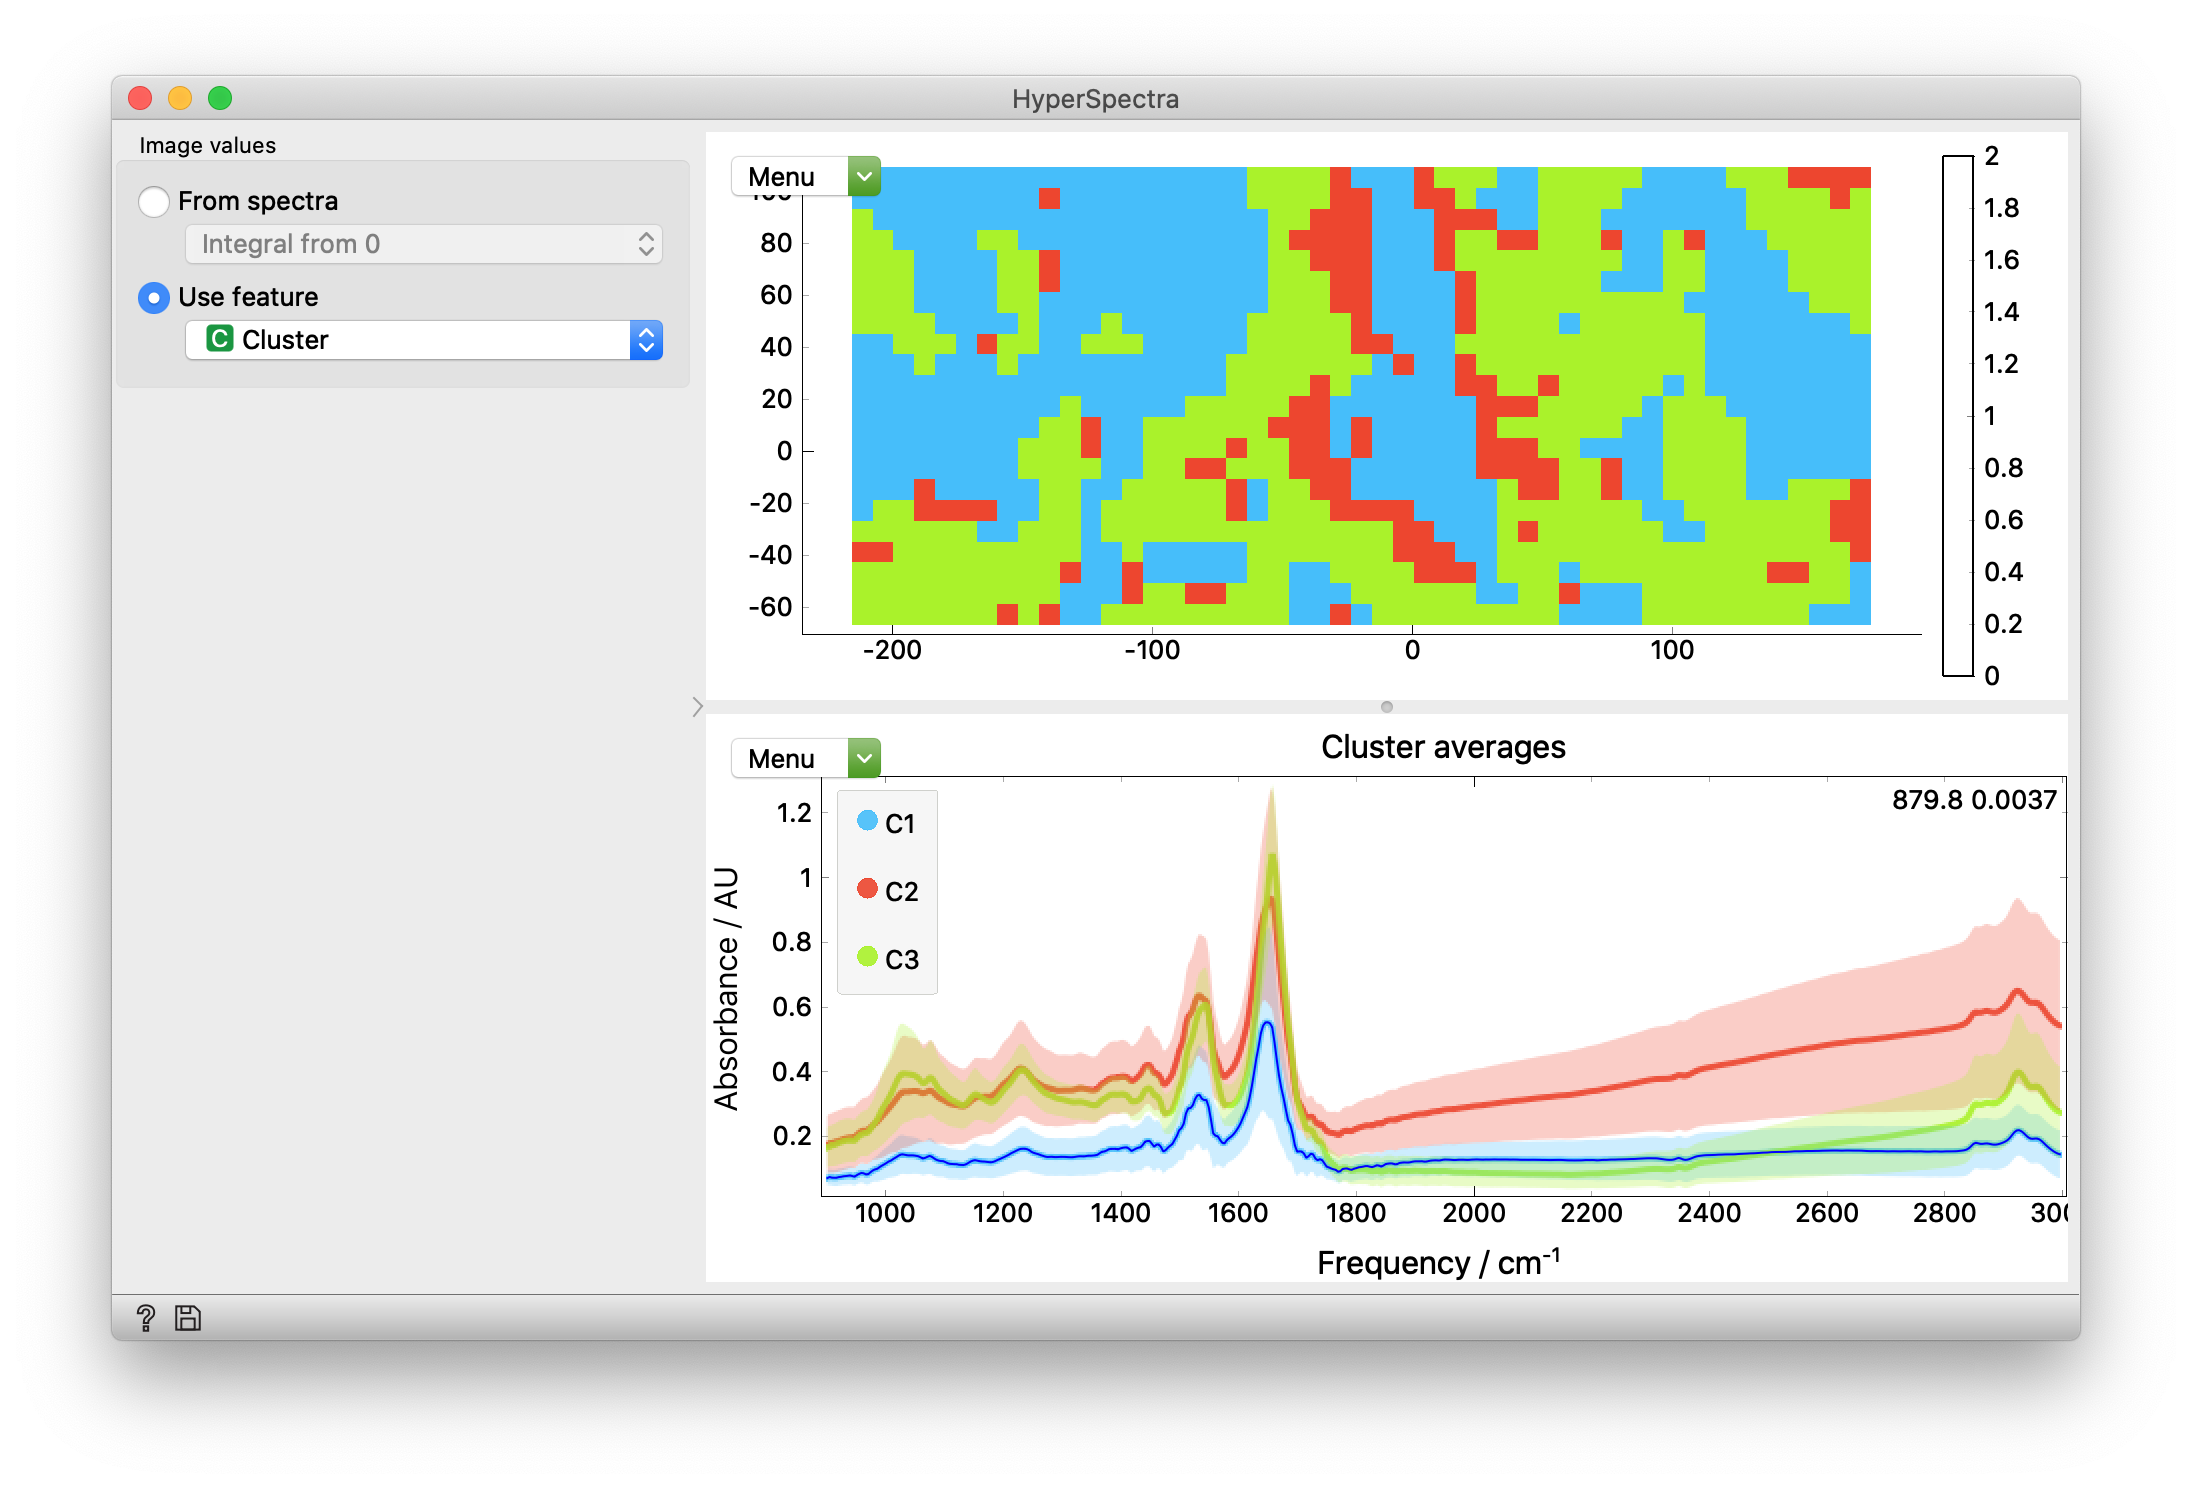
\includegraphics[scale=0.33]{graphics/ch-spectra_image_clustering/sp_image_clustering-fig2b.png}}
  {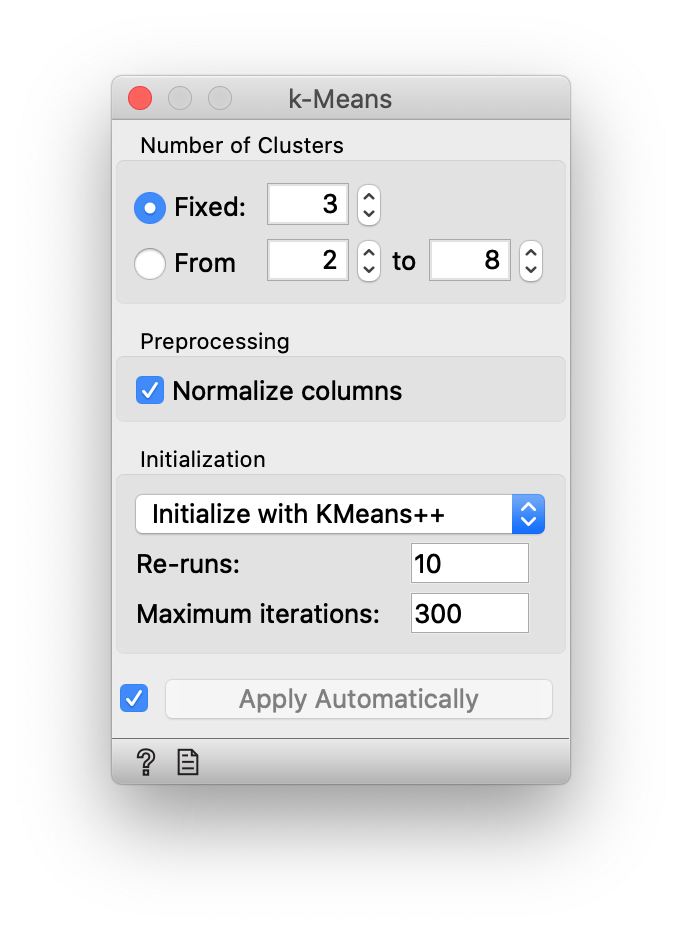
\includegraphics[scale=0.55]{graphics/ch-spectra_image_clustering/sp_image_clustering-fig2a.png}}
%  \caption{The \widget{Spectra} widget shows wrong predictions for the DNA class.}
  \label{ffig:spectra_image_clustering-fig2}
\end{figure}



\begin{wrapfigure}{o}{1.1\textwidth}
  \centering
  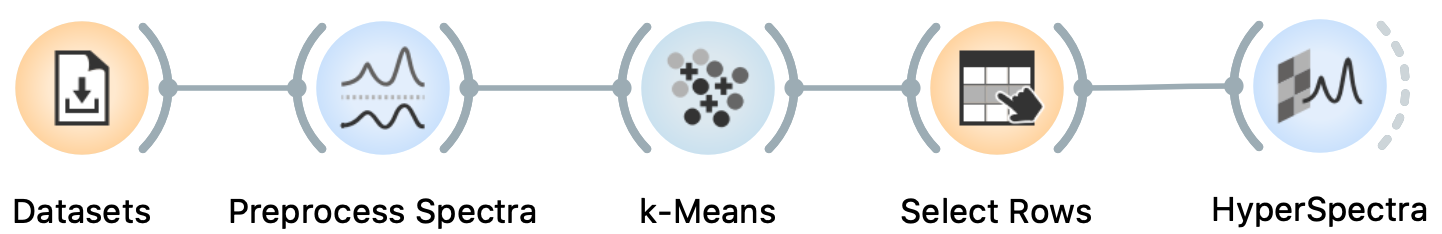
\includegraphics[width=1.1\textwidth]{graphics/ch-spectra_image_clustering/sp_image_clustering-fig3.png}%
  \label{fig:spectra_image_clustering-fig3}
\end{wrapfigure}
We see no meaningful clusters. Therefore, we need to preprocess the data. If we do it well, we see that a cluster corresponds to the background. We could remove it with the Select Rows widget.

\begin{wrapfigure}{o}{0.9\textwidth}
%  \centering
  \vspace{-0.5cm}
  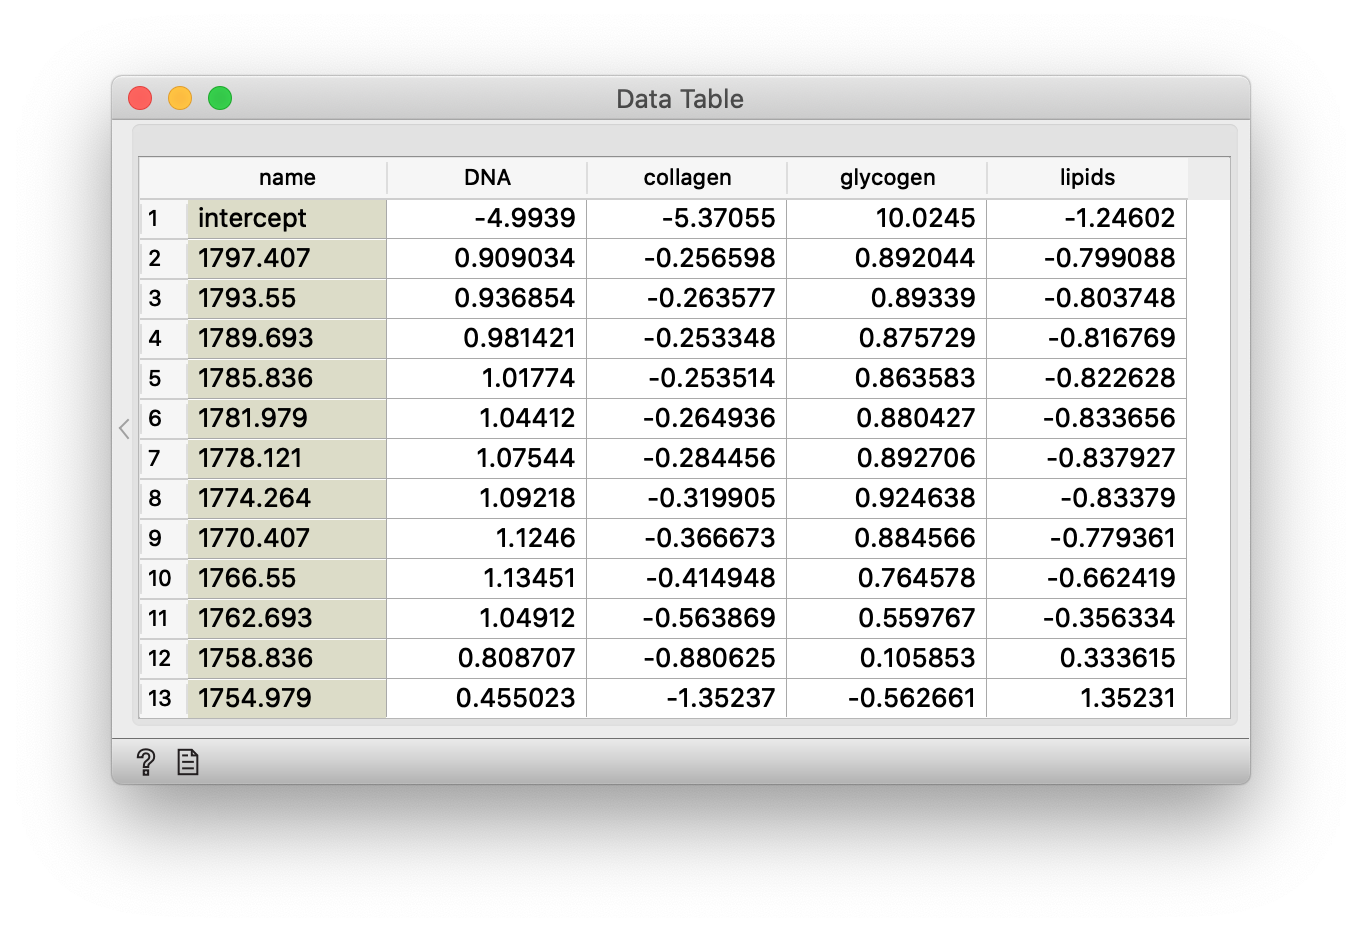
\includegraphics[width=0.9\textwidth]{graphics/ch-spectra_classification/sp_classification-fig4.png}
  \label{fig:spectra_classification-fig4}
\end{wrapfigure}
